\section{Creativity, Nonduality, Inspiration}

\begin{quotex}
The Genius is a man who discovers many others in himself. He is a man with many men in his personality. But then the genius can understand other men better than they can understand themselves, because within himself he has not only the character he is grasping, but also its opposite. Duality is necessary for observation and comprehension …in short, to understand man means to have equal parts of himself and his opposite in one. \flright{\textsc{Otto Weininger}}

\end{quotex}


Recently, we turned to \textbf{Boethius}\footnote{See Section \ref{sec:TheKnowerandtheKnown} in this book.} for an explanation of the types of knowledge: sensory and psychic impressions, rational thought, and intellectual intuition. Since intuition is what separates Tradition from philosophical or scientific systems, it is well worth the trouble to go over it again. A woman once told me that she has ``hunches" which she took to mean gnosis; of course, what we mean has nothing to do with so-called ``woman's intuition", but with a direct knowledge that brings absolute certainty.

\textbf{Vladimir Solovyov} relates intuition\footnote{See Section \ref{sec:OrganicandMechanicalThinking} in this book.} to ``an inner union of perfect individuality with complete generality or universality", and he points to the artist as the proof of intuition. That is because the artistic inspiration unites the concrete individual with its wholeness in the formless realm. This non-dual intuition differs from rational thinking which involves a subject and an object. \textbf{David Loy}, in his study of various teachings on Nonduality, refers to the personal experiences of several artists to demonstrate nondual thinking. However, artistic intuition is still not metaphysical realization or mystical intuition, since, as the examples will show, the artist is passive in relation to it and experiences it as an external force. Nevertheless, the examples are instructive and will help the reader become aware of his own everyday nondual experiences; for example, there may be that ``aha" moment of ``getting it" when the flow of the rational mind is temporarily halted.

\begin{wrapfigure}{rt}{.33\textwidth}
 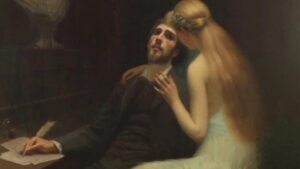
\includegraphics[scale=.5]{a20121204CreativityNondualityInspiration-img001.jpg} 
\caption{Leanan Sídhe}
\end{wrapfigure}

We have so many thoughts in a day that we usually take them for granted. We claim they are ``our" thoughts, or ``our" ideas. A little reflection will show that cannot be true. We don't know what we will think about one minute from now, as thoughts come from a source of their own against our will. Usually we become ``lost in thought", as thoughts link themselves together in an intricate story and take over our conscious mind and even feelings. Obviously, this inhibits metaphysical realization since the proper order of things is for the ``I" to dominate the other parts of conscious activity including the thought process. It is a good practice to sit quietly while trying to maintain a conscious detachment over the automatic processes of the mind. Then it will be possible to observe thoughts in their incipient stage. By maintaining conscious detachment, these thoughts will not be able to link and they will dissipate like wispy clouds in the wind. Otherwise, they will agglutinate into complex formations, and we will fantasize faces, things, and events as we usually do when staring at cloud formations in the sky.

Musical composition provides the easiest examples of artistic inspiration since it is the most abstract of the arts. The common experience is that the composition is grasped as a whole first, and only afterwards are the individual notes written down. This all-at-once feeling is what defines inspiration. In our spatial awareness, we are accustomed to grasping our field of sensory experience as a whole; however, it is more difficult to experience time that way. That is, how can the sequential elements of a temporal sequence be understood as a single whole? Yet, we do that all the time when we hear a symphony; although we experience each note and each instrument in time, we still grasp the symphony as a whole. We will have more to say about this when discussing how God can know the future.

I will let the artists speak for themselves. First we have \textbf{Mozart}:

\begin{quotex}
All this fires my soul and, provided I am not disturbed, my subject enlarges itself, becomes methodized and defined, and the whole, though it be long, stands almost complete and finished in my mind, so that I can survey it, like a fine picture or a beautiful statue, at a glance … All this inventing, this producing, takes place in a pleasing, lively dream. 

\end{quotex}
Loy points out that the subject enlarges or creates itself and it is dreamlike because there is no ``thinker" or directing ego. \textbf{Tchaikovsky}'s experience is similar:

\begin{quotex}
Generally speaking, the germ of a future composition comes suddenly and unexpectedly … It takes root with extraordinary force and rapidity, shoots up through the earth, puts forth branches and leaves, and finally blossoms. 

\end{quotex}
Some composers relate this to a religious experience. \textbf{Puccini} says:

\begin{quotex}
The music of this opera [Madam Butterfly] was dictated to me by God; I was merely instrumental in putting it on paper and communicating it to the public. 

\end{quotex}
\textbf{Wagner}'s experience is that:

\begin{quotex}
There are universal currents of Divine Thought vibrating the ether everywhere … I feel that I am one with this vibrating force. 

\end{quotex}
Finally, we need to hear what \textbf{Nietzsche} had to say:

\begin{quotex}
Has anyone at the end of the nineteenth century any distinct notion of what poets of a stronger age understood by the word inspiration?  If not, I will describe it. If you had the slightest residue of superstition left in you, it would hardly be possible to completely disregard the idea that one is the mere incarnation, a mouthpiece or a medium of an almighty power. The idea of revelation in the sense of something which profoundly moves and provokes, becoming suddenly visible and audible with indescribable certainty and accuracy—is a simple description. You hear — you do not seek; you take — and do not ask who gives: a thought suddenly flashes up like lightning, it comes as a necessity, without hesitation — I have never had any choice in the matter. There is an ecstasy so great that the immense strain of it is sometimes relaxed by a flood of tears during which one does not know whether one is coming or going. There is the feeling of completely being outside of oneself, with the very distinct consciousness of endless delicate shivers right down to one's toes; — there is a depth of happiness in which the most painful and gloomy parts do not detract from the whole but are produced and required as necessary shades of colour amidst such an overflow of light. There is an instinct for rhythmical relationships which embrace a whole world of forms: length, the need of an all-embracing rhythm, is almost the measure of the force of inspiration, a kind of compensation for its pressure and tension.



Everything happens quite involuntarily as if in a tempestuous outburst of freedom of absolute power and divinity. The involuntary nature of the images and similes is the most remarkable thing; one loses all perception of what is imagery and metaphor; everything seems to present itself in the readiest, the truest and simplest means of expression. It actually seems, to use one of Zarathustra's own phrases, as if all things came together and offered themselves as images 

\end{quotex}
Loy mentions several other poets, writers, and even mathematicians who have had similar experiences. Although Loy's primary focus is on nonduality as understood in Taoism, the Vedanta, and Buddhism, he does show how this is the same as intellectual intuition as understood by \textbf{Plotinus}, \textbf{Meister Eckhart}, \textbf{Nicolas of Cusa}, and \textbf{Boehme}.

\paragraph{Update 25 Feb 2021}

I spent 10 minutes searching for creativity. There are articles about how the neurons of creative people are different from the uncreative. As if neurons can create novelty out of nothing. The other modern view, completely opposed to the first, is that creativity can be taught to anyone at random.

If you think you are creative, do you understand any of quotes above? Creativity is dangerous: it is not a medical condition nor can you learn it at a weekend seminar. You need to surrender your imagination to forces whose source you neither know nor understand.


\flrightit{Posted on 2012-12-04 by Cologero }

\begin{center}* * *\end{center}

\begin{footnotesize}\begin{sffamily}

\texttt{Mihai on 2012-12-05 at 04:47 said: }

When I read words such as these from Nietzsche, I cannot help but wonder how he could be so unlike and above the mediocrity, bourgeois pettiness and socialist stupidity of his time, and yet be so completely immersed in the same roots from which the above mentioned sprung forth. 

When reading Nietzsche one gets this impression of a superior way of life, an iron discipline and a shinning intellect with outstanding intuitions (such as those quoted here). But then I can only wonder: what for ? All these great potential subjected to a complete dead end. Nietzsche's ``superman" is only a phantasm, an utopia in the same category with Marx's ``end of history". He had some pearls, but he couldn't find anything better to do with them but use them as food for swine. 

Sorry for my wandering off the topic. 

As for the mind, I have to say that trying to focus it is the same as trying to stabilize a ball on the peak of a cone. It stays there for a moment, but then immediately starts to fall towards the base. Even trying to be a silent witness to this process is difficult, as the ``I" is immediately attracted to identify with the flow of thought. But, then again, even the fact that one realizes all these facts proves that one, in a way, sees oneself as above and transcendes this very flow. It's a start.


\hfill

\texttt{Cologero on 2012-12-05 at 08:20 said: }

Yes, Mihai, since the conscious guard is let down in these stories of inspiration, then all sorts of spirits can be allowed in. We could just as easily post similar quotes from murderers and false prophets. The spirits must be tested.


\hfill

\texttt{Avery Morrow on 2012-12-05 at 08:58 said: }

To expand on that: when you admit the existence of good, you also admit the existence of evil. The whole point is that evil doesn't stand up with a big Nazi flag saying ``look how evil I am"; it uses the same techniques as good, and perverts them. Now, obviously, Nietzsche claimed to be above good and evil, but his own life is a kind of parable there… I'm going to quote from a memorable movie review I saw recently:

``He tried to fashion himself … above morality, above guilt, above society, immune to Christian charity, who could exercise his naked will to power, superior to all men who were constrained by mere values and compassion for their fellow man. So it is sadly and very fittingly ironic that Nietzsche, by expressing compassion for an abused horse, in the end himself broke down and gave into Christian pity, when all his life he claimed to be above and did all he could to negate such `weakness.'"


\hfill

\texttt{Cassiodorus on 2012-12-05 at 11:03 said: }

I'm not sure, but Nietzsche always struck me as a ``bizarro" Nagarjuna.


\hfill

\texttt{Mihai on 2012-12-06 at 03:29 said: }

Yes, no doubt.

CS Lewis put it very neatly when he said that ``the greatest sinners are made from the same fabric as the greatest saints"- understood in potential.


\hfill

\texttt{Senko on 2012-12-08 at 22:41 said: }

It also strikes me that quote from Nietzche, also strikes me the fact that it is usually quoted here. How can a man who got so many wonderful insights be so stranded as a whole / in the end? It's kind of Zygmunt Bauman, his analysis of modernity is perfect, his choice of countering it with Marxism is plain stupid, specially since his family had to fled the USSR. Returning to the topic at hand, those ``Aha!" moments are sweet, they are as the wind, they come and go as they please, but they better catch you working or praying!


\hfill


\end{sffamily}\end{footnotesize}
